In this section we will discuss the results, we will first look at them by language and then we will summarize all of the information.

\subsection{English}

The model results are summarized in \cref{tab:englishresults}. All the p-values indicate strong evidence against the null hypothesis with slightly different values for the different data sets.

\begin{table}[H]
    \centering
    \begin{tabular}{c|c|c|c|c}
        Prediction & Source & P-value & Slope & Intercept \\ \hline
        $l \sim \log i$ (character length) & CV & $<2.2e-16$ & 0.635 & 1.25 \\
        $l \sim -\log p$ (character length) & CV & $<2.2e-16$ & -0.492 & 7.774 \\
        $l \sim \log i$ (duration) & CV & $<2.2e-16$ & 0.055 & 0.045 \\
        $l \sim -\log p$ (duration) & CV & $<2.2e-16$ & -0.046 & 0.623 \\
        $l \sim \log i$ (character length) & PUD & $4.72e-13$ & 0.762 & 1.1 \\
        $l \sim -\log p$ (character length) & PUD & $2.9e-10$ & -0.897 & 10.706 \\
    \end{tabular}
    \caption{Prediction results for English}
    \label{tab:englishresults}
\end{table}

\begin{figure}[H]
    \centering
    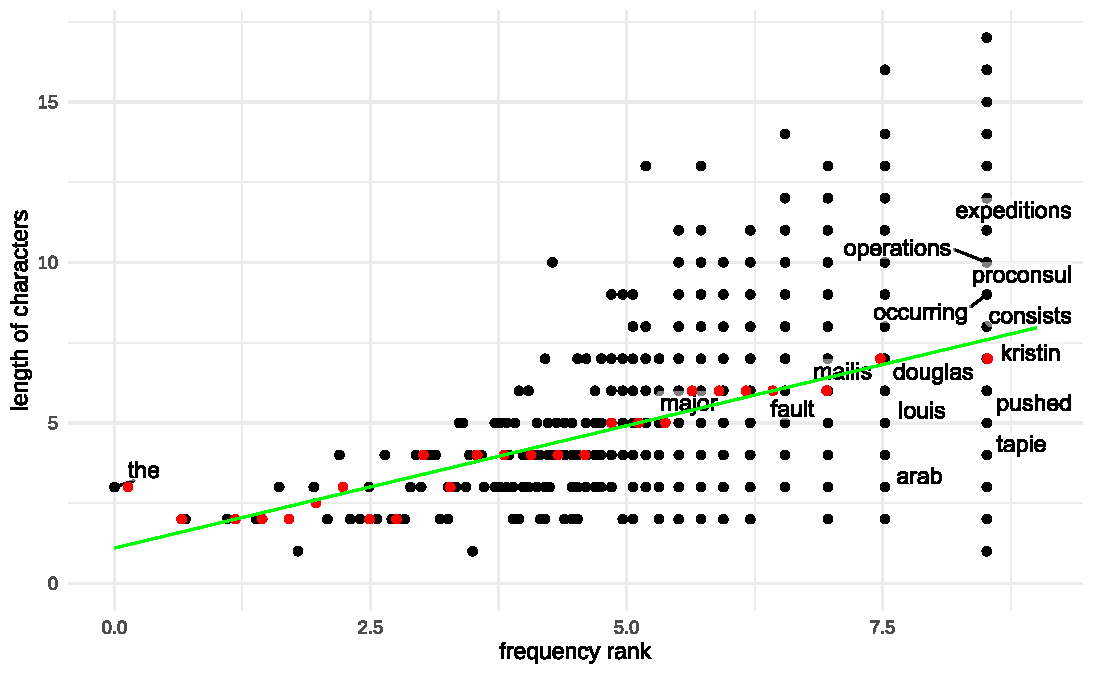
\includegraphics[width=0.6\textwidth]{plots/English_logi_cl_PUD.pdf}
    \caption{$l \sim \log i$ based on character length from PUD source plot for English}
    \label{english_logi_cl_PUD}
\end{figure}

\begin{figure}[H]
    \centering
    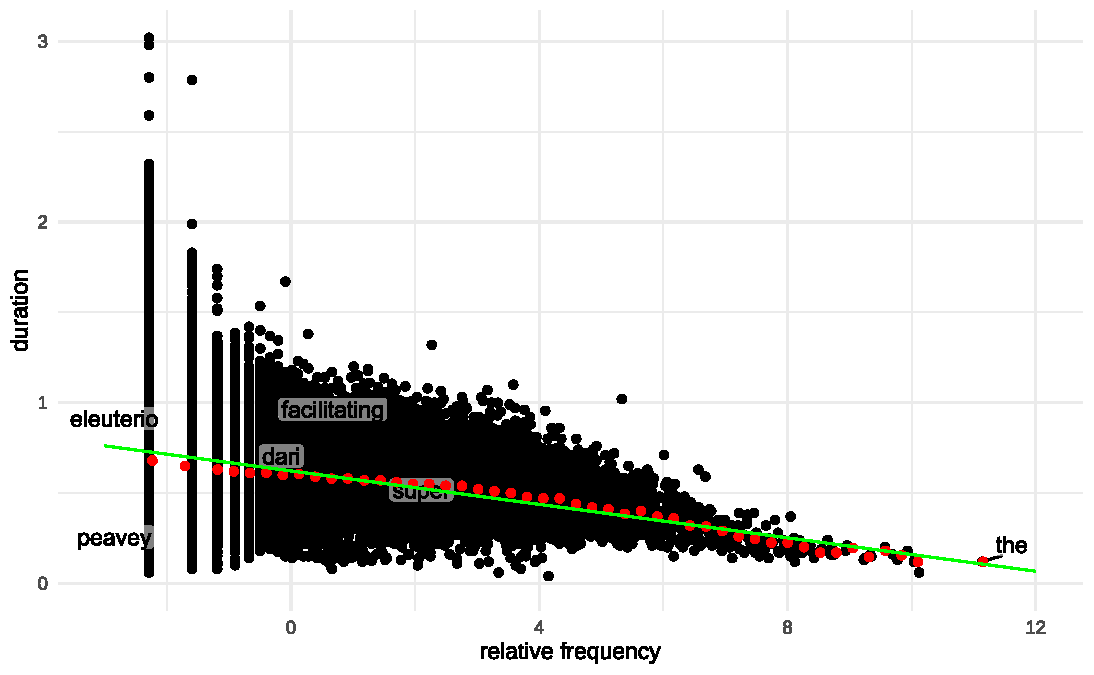
\includegraphics[width=0.6\textwidth]{plots/English_logp_d_CV.pdf}
    \caption{$l \sim \log i$ based on median duration from CV source plot for English}
    \label{english_logp_d_CV}
\end{figure}

In \cref{english_logi_cl_PUD} and \cref{english_logp_d_CV}, it can be seen how multiplicative binning is applied (in red) and robust linear regression is applied to the binned data to obtain the results.

\subsection{Spanish}

The model results are summarized in \cref{tab:spanishresults}. As for English, the p-values indicate strong evidence against the null hypothesis, and the predictions are similar too.

\begin{table}[H]
    \centering
    \begin{tabular}{c|c|c|c|c}
        Prediction & Source & P-value & Slope & Intercept \\ \hline
        $l \sim \log i$ (character length) & CV & $<2.2e-16$ & 0.655 & 1.725 \\
        $l \sim -\log p$ (character length) & CV & $<2.2e-16$ & -0.635 & 8.917 \\
        $l \sim \log i$ (duration) & CV & $<2.2e-16$ & 0.052 & 0.086 \\
        $l \sim -\log p$ (duration) & CV & $<2.2e-16$ & -0.050 & 0.670 \\
        $l \sim \log i$ (character length) & PUD & $1.27e-14$ & 0.866 & 0.955 \\
        $l \sim -\log p$ (character length) & PUD & $1.31e-12$ & -0.88 & 11.115 \\
    \end{tabular}
    \caption{Prediction results for Spanish}
    \label{tab:spanishresults}
\end{table}

\begin{figure}[H]
    \centering
    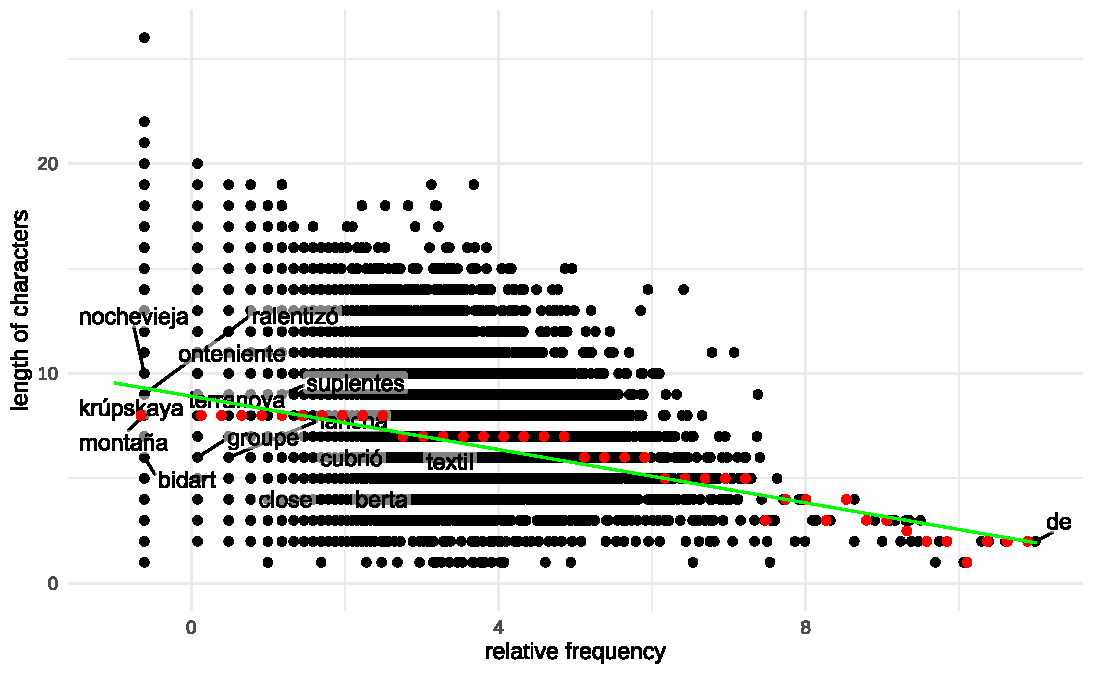
\includegraphics[width=0.6\textwidth]{plots/Spanish_logp_cl_CV.pdf}
    \caption{$l \sim -\log p$ based on character length from CV source plot for Spanish}
    \label{spanish_logp_cl_CV}
\end{figure}

In \cref{spanish_logp_cl_CV}, like for English, we can visually see the effects of the statistical analysis, but this time for $l \sim -\log p$ based on character length.

\subsection{Catalan}

The model results are summarized in \cref{tab:catalanresults}. As for the previous two languages, the p-values indicate strong evidence against the null hypothesis, and the predictions are similar as well.

\begin{table}[H]
    \centering
    \begin{tabular}{c|c|c|c|c}
        Prediction & Source & P-value & Slope & Intercept \\ \hline
        $l \sim \log i$ (character length) & CV & $<2.2e-16$ & 0.762 & 0.7 \\
        $l \sim -\log p$ (character length) & CV & $<2.2e-16$ & -0.693 & 9.09 \\
        $l \sim \log i$ (duration) & CV & $<2.2e-16$ & 0.061 & 0.036 \\
        $l \sim -\log p$ (duration) & CV & $<2.2e-16$ & -0.057 & 0.698 \\
    \end{tabular}
    \caption{Prediction results for Catalan}
    \label{tab:catalanresults}
\end{table}

\subsection{Arabic}

Arabic is the first language that had not been analyzed before in previous research \cite{torre2019physical} \cite{hernandez2019linguistic}. Once again, as can be seen in \cref{tab:arabicresults}, the p-values indicate strong evidence against the null hypothesis, and the predictions, although less than in the previous languages, look similar to the previous ones.

\begin{table}[H]
    \centering
    \begin{tabular}{c|c|c|c|c}
        Prediction & Source & P-value & Slope & Intercept \\ \hline
        $l \sim \log i$ (character length) & CV & $5.08e-14$ & 0.401 & 1.737 \\
        $l \sim -\log p$ (character length) & CV & $1.76e-12$ & -0.476 & 6.938 \\
        $l \sim \log i$ (duration) & CV & $5.17e-15$ & 0.052 & 0.916 \\
        $l \sim -\log p$ (duration) & CV & $1.9e-12$ & -0.064 & 0.86 \\
        $l \sim \log i$ (character length) & PUD & $1.58e-11$ & 0.635 & 0.917 \\
        $l \sim -\log p$ (character length) & PUD & $5.06e-11$ & -0.726 & 8.714 \\
    \end{tabular}
    \caption{Prediction results for Arabic}
    \label{tab:arabicresults}
\end{table}

\subsection{Indonesian}

Indonesian is the first language from the Austronesian family, and, like Arabic, regardless of being from a different language family than the previous, the p-values indicate strong evidence against the null hypothesis, and the predictions also look similar to the previous ones. The results can be seen in \cref{tab:indonesianresults}.

\begin{table}[H]
    \centering
    \begin{tabular}{c|c|c|c|c}
        Prediction & Source & P-value & Slope & Intercept \\ \hline
        $l \sim \log i$ (character length) & CV & $2.6e-11$ & 0.635 & 2.25 \\
        $l \sim -\log p$ (character length) & CV & $5.82e-11$ & -0.663 & 10 \\
        $l \sim \log i$ (duration) & CV & $2.41e-13$ & 0.046 & 0.16 \\
        $l \sim -\log p$ (duration) & CV & $1.58e-11$ & -0.047 & 0.716 \\
        $l \sim \log i$ (character length) & PUD & $6.21e-10$ & 0.545 & 3.071 \\
        $l \sim -\log p$ (character length) & PUD & $2.65e-06$ & -0.635 & 10.25 \\
    \end{tabular}
    \caption{Prediction results for Indonesian}
    \label{tab:indonesianresults}
\end{table}

\subsection{Turkish}

Turkish is, once again, the first language of a new family, in this case, the Turkic. Similar to the previous ones, regardless of being from a different language family than the previous, the p-values indicate strong evidence against the null hypothesis, and the predictions also look similar to the previous ones as can be seen in\cref{tab:turkishresults}.

\begin{table}[H]
    \centering
    \begin{tabular}{c|c|c|c|c}
        Prediction & Source & P-value & Slope & Intercept \\ \hline
        $l \sim \log i$ (character length) & CV & $<2.2e-16$ & 0.762 & 1.5 \\
        $l \sim -\log p$ (character length) & CV & $<2.2e-16$ & -0.866 & 11.045 \\
        $l \sim \log i$ (duration) & CV & $<2.2e-16$ & 0.052 & 0.102 \\
        $l \sim -\log p$ (duration) & CV & $<2.2e-16$ & -0.057 & 0.748 \\
        $l \sim \log i$ (character length) & PUD & $2.14e-08$ & 0.635 & 1.917 \\
        $l \sim -\log p$ (character length) & PUD & $3.16e-08$ & -0.953 & 11.5 \\
    \end{tabular}
    \caption{Prediction results for Turkish}
    \label{tab:turkishresults}
\end{table}

\subsection{Chinese}

Chinese is also a language from a new family, the Sino-Tibetan, and because of its representation, its case is different than previous languages. We analyzed the data basing character length on pinyin character length (the romanized version of Chinese characters), Chinese characters strokes, and Chinese characters length. This time around, the data looks different in some cases and even shows opposite trends as in previous languages. Nonetheless, the p-values still indicate strong evidence against the null hypothesis, which means that there is a statistical relationship. The data can be seen in \cref{tab:chineseresults}.

\begin{table}[H]
    \centering
    \begin{tabular}{c|c|c|c|c}
        Prediction & Source & P-value & Slope & Intercept \\ \hline
        $l \sim \log i$ (pinyin character length) & PUD & $0.0006232$ & -1.271 & 13 \\
        $l \sim -\log p$ (pinyin character length) & PUD & $0.004781$ & 3.15 & -10.375 \\
        $l \sim \log i$ (character length) & PUD & $5.53e-05$ & 0.136 & 0.839 \\
        $l \sim -\log p$ (character length) & PUD & $5.2e-05$ & -0.173 & 2.75 \\
        $l \sim \log i$ (strokes) & PUD & $4.23e-05$ & -6.353 & 73.417 \\
        $l \sim -\log p$ (strokes) & PUD & $0.0002516$ & 26.408 & -115.464 \\
    \end{tabular}
    \caption{Prediction results for Chinese}
    \label{tab:chineseresults}
\end{table}

When looking at the data from \cref{chinese_logi_cl_PUD_pinyin} and \cref{chinese_logi_cl_PUD_pinyin}, we can see the inverse correlation when word length is measured by pinyin character length. For $l \sim \log i$, the relationship is negative rather than positive as we had seen until now, therefore it is $l \sim -\log i$. The same thing happens for $l \sim -\log p$, which in this case appears to be $l \sim \log p$. Both show a significantly bigger slope than compared to the other languages.

\begin{figure}[H]
    \centering
    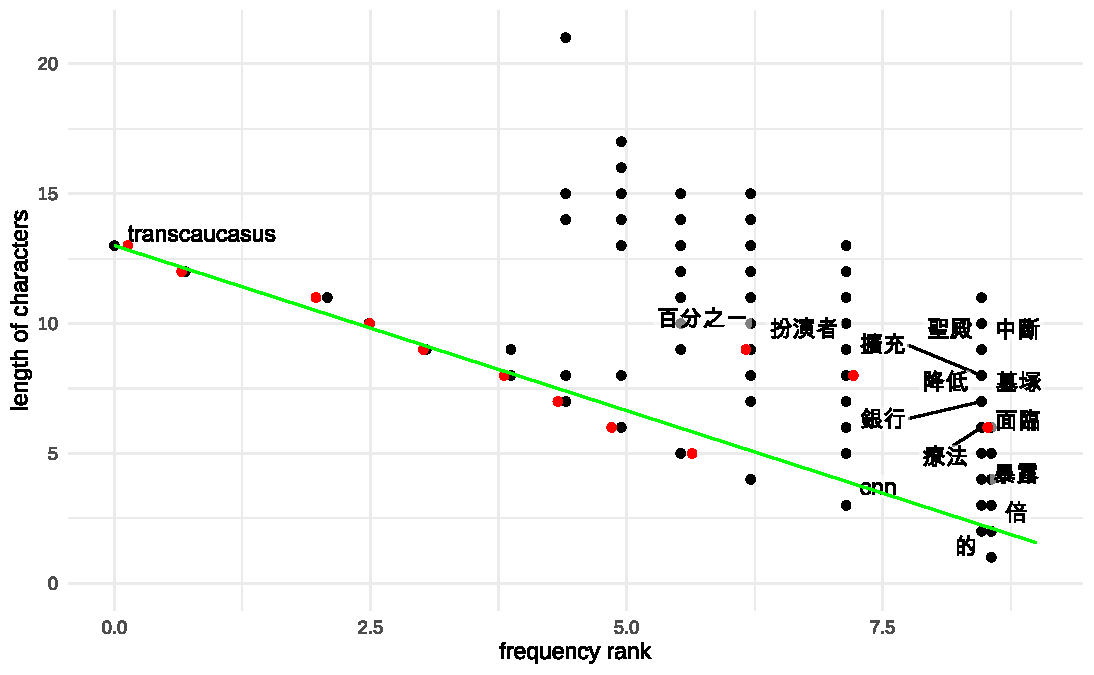
\includegraphics[width=0.6\textwidth]{plots/Chinese_logi_cl_PUD_pinyin.pdf}
    \caption{$l \sim \log i$ based on pinyin character length from PUD source plot for Chinese}
    \label{chinese_logi_cl_PUD_pinyin}
\end{figure}

\begin{figure}[H]
    \centering
    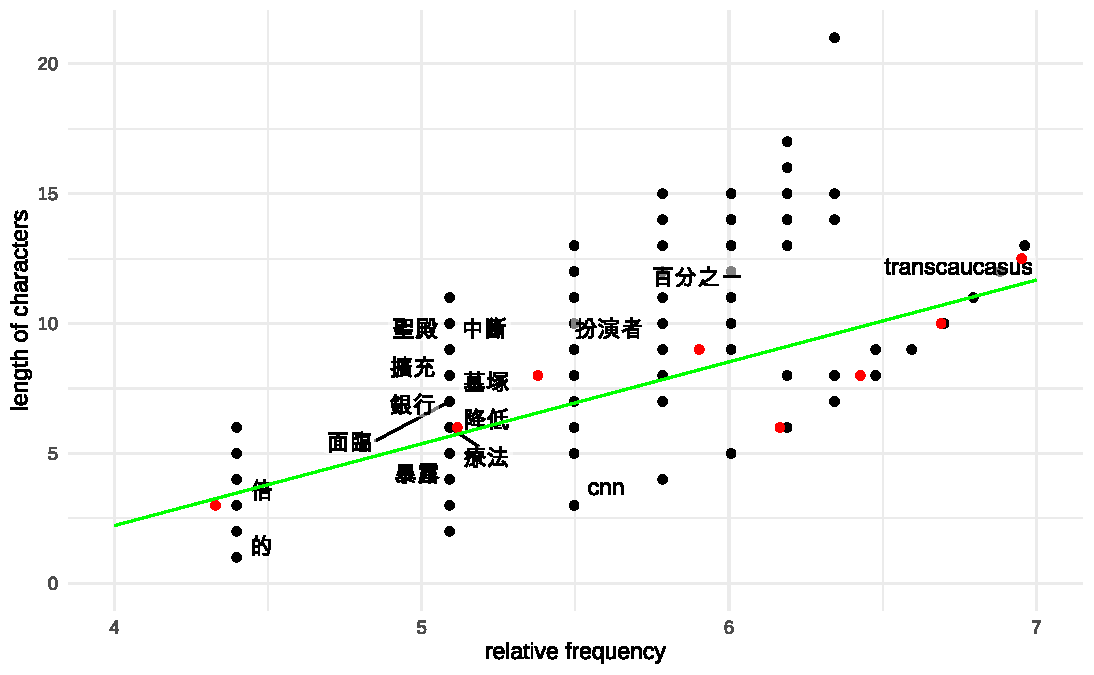
\includegraphics[width=0.6\textwidth]{plots/Chinese_logp_cl_PUD_pinyin.pdf}
    \caption{$l \sim -\log p$ based on pinyin character length from PUD source plot for Chinese}
    \label{chinese_logp_cl_PUD_pinyin}
\end{figure}

Instead, if we look at Chinese character length, the data is similar to the rest of the languages. But again, when looking at strokes in \cref{chinese_logi_cl_PUD_strokes} and \cref{chinese_logp_cl_PUD_strokes}, the relationship is also opposed to the trend we had observed until now, and this time with much bigger slope and intercept values probably due to the greater amount of strokes in words compared to the number of Latin characters in words from the other languages.

\begin{figure}[H]
    \centering
    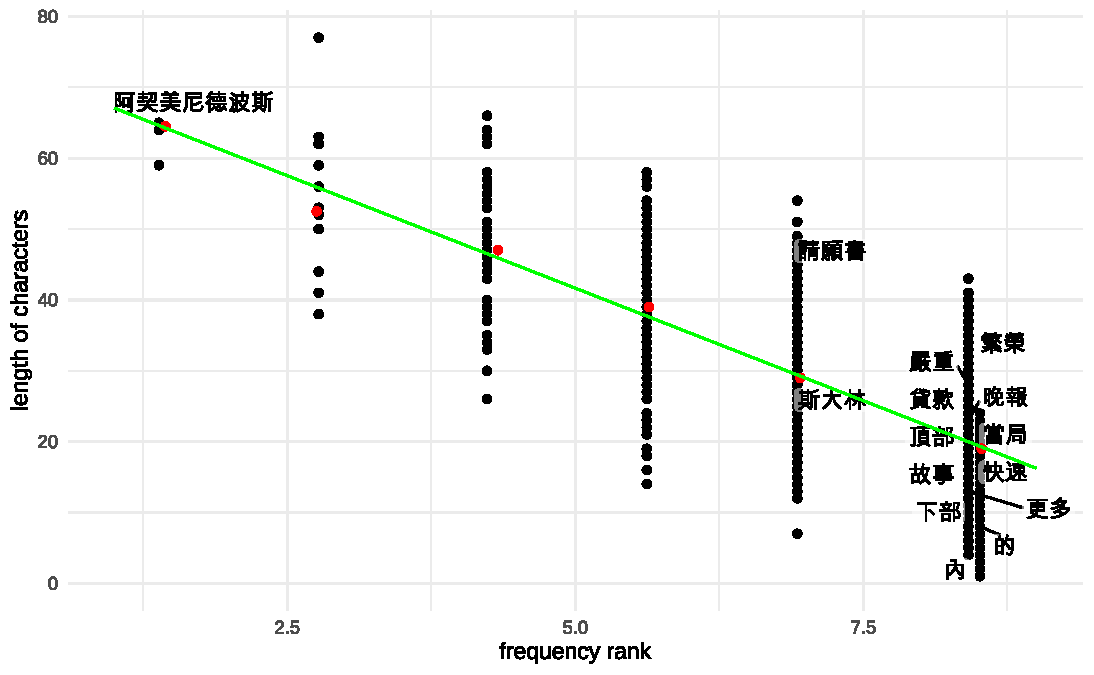
\includegraphics[width=0.6\textwidth]{plots/Chinese_logi_cl_PUD_strokes.pdf}
    \caption{$l \sim \log i$ based on strokes from PUD source plot for Chinese}
    \label{chinese_logi_cl_PUD_strokes}
\end{figure}

\begin{figure}[H]
    \centering
    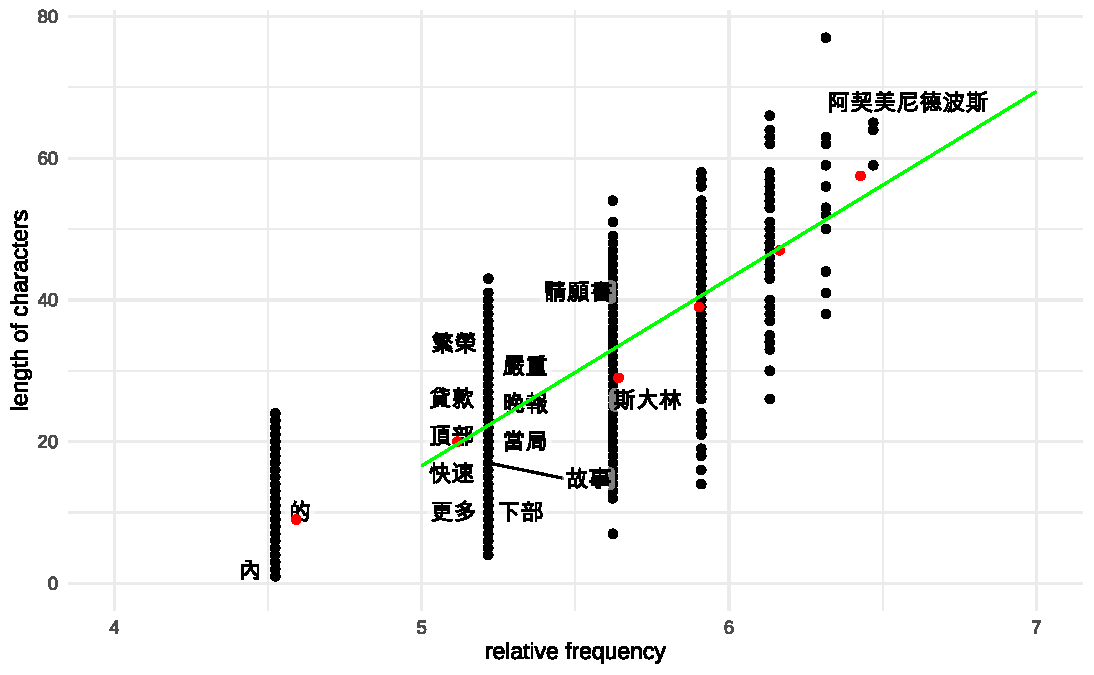
\includegraphics[width=0.6\textwidth]{plots/Chinese_logp_cl_PUD_strokes.pdf}
    \caption{$l \sim -\log p$ based on strokes from PUD source plot for Chinese}
    \label{chinese_logp_cl_PUD_strokes}
\end{figure}

\subsection{Tamil}

Given the case of Chinese, it is interesting to look at Tamil, which is another language that does not have a Latin script. As for the case of Arabic, we see that in Tamil the p-values indicate strong evidence against the null hypothesis, and the data also looks more similar to the majority of the analyzed languages. The data can be seen in \cref{tab:tamilresults}.

\begin{table}[H]
    \centering
    \begin{tabular}{c|c|c|c|c}
        Prediction & Source & P-value & Slope & Intercept \\ \hline
        $l \sim \log i$ (character length) & CV & $8.06e-05$ & 0.52 & 3.068 \\
        $l \sim -\log p$ (character length) & CV & $3.97e-06$ & -0.635 & 10.083 \\
        $l \sim \log i$ (duration) & CV & $2.79e-05$ & 0.044 & 0.323 \\
        $l \sim -\log p$ (duration) & CV & $4.9e-06$ & -0.061 & 0.969 \\
    \end{tabular}
    \caption{Prediction results for Tamil}
    \label{tab:tamilresults}
\end{table}

\subsection{Basque}

Basque is a different case since it is a language that does not have a family, but still, we can observe the same pattern as with the previous languages. The p-values indicate strong evidence against the null hypothesis, and the slopes and intercept follow the same pattern as the previous languages. The data can be seen in \cref{tab:basqueresults}.

\begin{table}[H]
    \centering
    \begin{tabular}{c|c|c|c|c}
        Prediction & Source & P-value & Slope & Intercept \\ \hline
        $l \sim \log i$ (character length) & CV & $<2.2e-16$ & 0.762 & 1.7 \\
        $l \sim -\log p$ (character length) & CV & $<2.2e-16$ & -0.794 & 10.646 \\
        $l \sim \log i$ (duration) & CV & $<2.2e-16$ & 0.051 & 0.126 \\
        $l \sim -\log p$ (duration) & CV & $<2.2e-16$ & -0.055 & 0.74 \\
    \end{tabular}
    \caption{Prediction results for Basque}
    \label{tab:basqueresults}
\end{table}

\subsection{Summary}

As can be seen in \cref{tab:logi_cl}, all languages except for Chinese have a slope value between 0.4 and 0.8 and intercept between 0.7 and 3, so not only all of them have the same. In the case of Chinese, the characters version did follow the same trend with a smaller scope, but the the pinyin characters and strokes versions had an inverse trend.

\begin{table}[H]
    \centering
    \begin{tabular}{c|c|c|c}
        Language & $l \sim \log i$ CV & $l \sim \log i$ PUD & $l \sim \log i$ Average \\ \hline
        English & $0.635*x + 1.25$ & $0.762*x + 1.1$ & $0.7*x + 1.175$ \\
        Spanish & $0.655*x + 1.725$ & $0.866*x + 0.955$ & $0.761*x + 1.34$ \\
        Catalan & $0.762*x + 0.7$ & N/A & $0.762*x + 0.7$ \\
        Arabic & $0.401*x + 1.737$ & $0.635*x + 0.917$ & $0.518*x + 1.327$ \\
        Indonesian & $0.635*x + 2.25$ & $0.545*x + 3.071$ & $0.59*x + 2.661$ \\
        Turkish & $0.762*x + 1.5$ & $0.635*x + 1.917$ & $0.7*x + 1.709$ \\
        Chinese (pinyin) & N/A & $-1.271*x + 13$ & $-1.271*x + 13$ \\
        Chinese (characters) & N/A & $0.136*x + 0.839$ & $0.136*x + 0.839$ \\
        Chinese (strokes) & N/A & $-6.353*x + 73.417$ & $-6.353*x + 73.417$ \\
        Tamil & $0.52*x + 3.068$ & N/A & $0.52*x + 3.068$ \\
        Basque & $0.762*x + 1.7$ & N/A & $0.762*x + 1.7$ \\
    \end{tabular}
    \caption{Summary of $l \sim \log i$ results for character length}
    \label{tab:logi_cl}
\end{table}

For the case of duration as length, as can be seen in \cref{tab:logi_d}, all the slope values are between 0.04 and 0.06, and all intercept values are between 0 and 1. In this case, there is no data for Chinese, so the data appears to be very similar to the character length one, where all languages had a positive correlation with similar slope and intercept values.

\begin{table}[H]
    \centering
    \begin{tabular}{c|c}
        Language & $l \sim \log i$ CV \\ \hline
        English & $0.055*x + 0.045$ \\
        Spanish & $0.052*x + 0.086$ \\
        Catalan & $0.061*x + 0.036$ \\
        Arabic & $0.052*x + 0.916$ \\
        Indonesian & $0.046*x + 0.16$ \\
        Turkish & $0.052*x + 0.102$ \\
        Tamil & $0.044*x + 0.323$ \\
        Basque & $0.051*x + 0.126$ \\
    \end{tabular}
    \caption{Summary of $l \sim \log i$ results for duration}
    \label{tab:logi_d}
\end{table}

If we look at data for $l \sim -\log p$ based on character length in \cref{tab:logp_cl}, we see that once again, all languages except for Chinese look similar with a slope between 0.4 and 0.95 and an intercept value between 6.9 and 11.1. For Chinese, we also observe that only the version that uses Chinese characters for word length gets a negative correlation like for the rest of the data but with different values, and the pinyin and stroke versions have an inverse correlation compared to the rest, in this case, a positive one.

\begin{table}[H]
    \centering
    \begin{tabular}{c|c|c|c}
        Language & $l \sim -\log p$ CV & $l \sim -\log p$ PUD & $l \sim -\log p$ Average \\ \hline
        English & $-0.492*x + 7.774$ & $-0.897*x + 10.706$ & $-0.695*x + 9.24$ \\
        Spanish & $-0.635*x + 8.917$ & $-0.88*x + 11.115$ & $-0.758*x + 10.016$ \\
        Catalan & $-0.693*x + 9.09$ & N/A & $-0.693*x + 9.09$ \\
        Arabic & $-0.476*x + 6.938$ & $-0.726*x + 8.714$ & $-0.601*x + 7.826$ \\
        Indonesian & $-0.663*x + 10$ & $-0.635*x + 10.25$ & $-0.649*x + 10.125$ \\
        Turkish & $-0.866*x + 11.045$ & $-0.953*x + 11.5$ & $-0.91*x + 11.273$ \\
        Chinese (pinyin) & N/A & $3.15*x + -10.375$ & $3.15*x + -10.375$ \\
        Chinese (characters) & N/A & $-0.173*x + 2.75$ & $-0.173*x + 2.75$ \\
        Chinese (strokes) & N/A & $26.408*x - 115.464$ & $26.408*x - 115.464$ \\
        Tamil & $-0.635*x + 10.083$ & N/A & $-0.635*x + 10.083$ \\
        Basque & $-0.794*x + 10.646$ & N/A & $-0.794*x + 10.646$ \\
    \end{tabular}
    \caption{Summary of $l \sim -\log p$ results for character length}
    \label{tab:logp_cl}
\end{table}

In the data for word length as duration shown in \cref{tab:logp_d}, we see that, once again, all languages follow the same pattern, all slope values are between 0.04 and 0.07 and all intercept values are between 0.6 and 1.

\begin{table}[H]
    \centering
    \begin{tabular}{c|c}
        Language & $l \sim \log i$ CV \\ \hline
        English & $-0.046*x + 0.623$ \\
        Spanish & $-0.050*x + 0.670$ \\
        Catalan & $-0.057*x + 0.698$ \\
        Arabic & $-0.064*x + 0.86$ \\
        Indonesian & $-0.047*x + 0.716$ \\
        Turkish & $-0.057*x + 0.748$ \\
        Tamil & $-0.061*x + 0.969$ \\
        Basque & $-0.055*x + 0.74$ \\
    \end{tabular}
    \caption{Summary of $l \sim -\log p$ results for duration}
    \label{tab:logp_d}
\end{table}

All of the plots generated can be found in \cref{sec:annex}.